\section{Coverage}\label{sec:startnodecoverage}

File \code{coverage.ipynb} contains the histograms for the coverage obtained
with the configuration named ``StartNodePosition''. All parameters have been
fixed and we have performed 200 experiments with the starting user at the
center, border and corner --- for a total of 600 experiments.

The notebook also shows statistics about the coverage in the three cases.
Results are shown in \tableref{table:startnodecoveragestats}.

\begin{table}[hbt]
	\centering
	\begin{tabular}{lcccc}
		\toprule
		Start Node Pos\@. & Mean & Std\@. Dev\@. & Min\@. & Max\@. \\
		\midrule
		Center & \makecell[c]{\(1235.785\) \\ (\(98.942\%\))}
		       & \makecell[c]{\(7.084471\) \\ (\(0.5672\%\))}
		       & \makecell[c]{\(1213\) \\ (\(97.1177\%\))}
		       & \makecell[c]{\(1248\) \\ (\(99.9199\%\))} \\[16pt]
		Border & \makecell[c]{\(1225.345\) \\ (\(98.1061\%\))}
		       & \makecell[c]{\(123.317566\) \\ (\(9.8733\%\))}
		       & \(0\)
		       & \makecell[c]{\(1248\) \\ (\(99.9199\%\))} \\[16pt]
		Corner & \makecell[c]{\(910.64\) \\ (\(72.9095\%\))}
		       & \makecell[c]{\(546.580205\) \\ (\(43.7614\%\))}
		       & \(0\)
		       & \makecell[c]{\(1248\) \\ (\(99.9199\%\))} \\
		\bottomrule
	\end{tabular}
	\caption{Statistics about coverage when the starting node is in the
	center/border/corner (low density
	condition)}\label{table:startnodecoveragestats}
\end{table}

As we can see, the mean is higher if the starting user is positioned in the
center and lower if it is positioned in the border or corner. Additionally we
have higher standard deviations when the starting user is moved near the corner.
When the starting user is in the center, we have are able to guarantee a
coverage of at least \(97\%\) with \(R\!=\!25m\) in low density conditions,
while when the starting user is placed at the border or the corner the coverage
can drop down to zero.

Files \code{\{low,high\}-density-coverage.ipynb} contain the analysis of the
coverage in the two conditions (low density and high density) when the radius is
varied from very low values to high values. Data has been collected using the
configurations named ``StartNodePositionLowDensity'' and
``StartNodePositionHighDensity''.

\figref{subfig:ldstartnodecoverage} shows the results for the low density
case\footnote{For easier visualization, the Jupyter notebook also contains the
same data plotted in three different figures rather than with the center, border
and corner cases in the same plot.}. As we can see, in the ``center'' case the
mean coverage starts very high even with low values of \(R\): The minimum mean
is around \(1150\) (from a total of \(1249\) reachable users) and it stabilizes
near the value \(1240\) for \(R \ge 25m\).

\begin{figure}[hbt]
	\centering
	\begin{subfigure}[b]{0.49\textwidth}
		\centering
		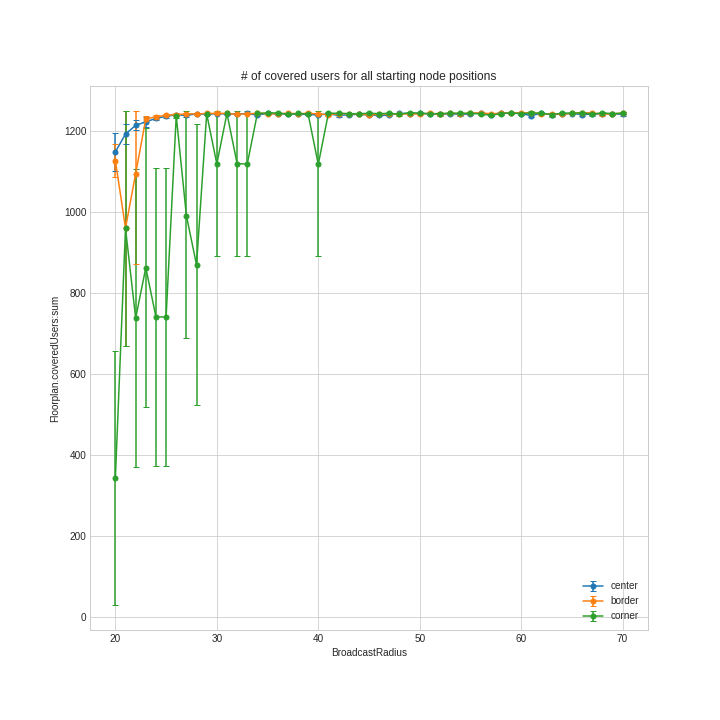
\includegraphics[width=\textwidth]{img/ld/start-node-coverage}
		\caption{Low density scenario}\label{subfig:ldstartnodecoverage}
	\end{subfigure}
	\begin{subfigure}[b]{0.49\textwidth}
		\centering
		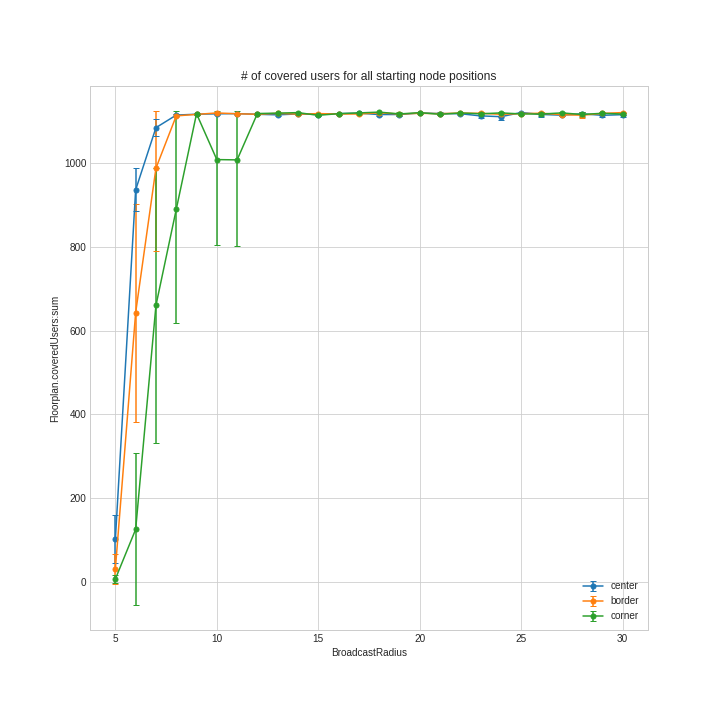
\includegraphics[width=\textwidth]{img/hd/start-node-coverage}
		\caption{High density
		scenario}\label{subfig:hdstartnodecoverage}
	\end{subfigure}
	\caption{For low values of \(R\), the coverage is generally worse if the
	starting node is in the corner rather than in the
	center}\label{fig:startnodepositioncoverage}
\end{figure}

Also in the ``border'' case the coverage stabilizes at high values with \(R \ge
25m\), but it has very high variance when the broadcast radius is very low and
it also happens that the first user sending the message is not able to reach
anyone, giving a coverage of zero.

In the ``corner'' case the situation is even worse: up until \(R \le 33m\) we
do not have a stable coverage and even after we get lower mean with a huge
variance with \(R\!=\!40m\). As we can see from the table at the end of the
notebook, this is due to a catastrophic experiment where the starting user has
not reached any user even with \(R\!=\!40m\).

\figref{subfig:hdstartnodecoverage} shows the results for the high density
scenario. Considerations are the same done for the low density scenario, so we
will not discuss the results here.

So, if possible, when designing a network of this type, to guarantee a nearly
perfect coverage, we should try to ensure that the starting user is near as much
as possible to the center or, at least, avoid the corners of the floorplan. If
this is not possible, to guarantee\footnote{With ``guarantee'' we do not mean a
100\% guarantee, of course: more experiments are needed to explore more
possibilities and, with the total randomness on the position of the users, the
only values of the broadcast radius that \emph{really} guarantees a coverage
greater than zero are those values that always make the starting user to reach
the entire floorplan immediately. Values found (\(40m\) and \(11m\)) are only an
\emph{hint} of minimum values that makes \emph{hard} to get a catastrophic
situation.} the coverage, it is necessary to increase the broadcast radius (\(R
> 40m\) for low density; \(R > 11m\) for high density).

The probability to found a user inside the area of reachability of the starting
node \idest{the probability to get a coverage greater than 0} can be easily
computed, in the general case, with~\eqref{eq:nocatastropheprobability}. The
equation has been derived by considering the inverse of the probability to found
\idest{the probability to \emph{not} found any node in the area of reachability,
which is the probability to found all the nodes in the area outside the area of
reachability} which is, for a single user, the area of reachability
(\(\alpha\cdot\pi\cdot R^2\)) divided by the area of the floorplan (\(X\cdot
Y\)). This probability has been then extended to the case of \(N\) users by
raising it to the number of users except the first one (\(N-1\)).

\begin{equation}\label{eq:nocatastropheprobability}
	P = 1 - {\left(\frac{\alpha\pi R^2}{XY}\right)}^{N-1}
\end{equation}

We can verify that for \(R\!=\!40m\), \(N\!=\!1250\), \(X\!=\!Y\!=\!500m\), with
the starting node in the corner (\(\alpha\!=\!\frac{1}{4}\)), we get:

\[
	P = 1 -
	{\left(\frac{\frac{1}{4}\pi\cdot40^2}{500\cdot500}\right)}^{1249} \simeq
	99.4973\%
\]

which is a quite high probability. Only in just \(\frac{1}{200}\) cases we will
get a coverage equal to zero in the case of the low density scenario with
\(R\!=\!40m\).
